\let\negmedspace\undefined
\let\negthickspace\undefined
\documentclass[a4,12pt,onecolumn]{IEEEtran}
\usepackage{amsmath,amssymb,amsfonts,amsthm}
\usepackage{algorithmic}
\usepackage{graphicx}
\usepackage{textcomp}
\usepackage{xcolor}
\usepackage{txfonts}
\usepackage{listings}
\usepackage{enumitem}
\usepackage{mathtools}
\usepackage{gensymb}
\usepackage[breaklinks=true]{hyperref}
\usepackage{tkz-euclide}
\usepackage{listings}
\usepackage{circuitikz}
\usepackage{gvv}
\begin{document}
\title{
\Huge\textbf{ Discrete Assignment} \\
\textbf{NCRET - 10.5.3.11}
\author{Shravya Kantayapalam \\EE23BTECH11030}}
\maketitle
\textbf{Question} 
 If the sum of the first $ n $ terms of an AP is $4n - n^2$, what is the first term ($ S_1 $)? What is the sum of the first two terms? What is the second term? Similarly, find the 3rd, the 10th, and the $n$th terms.
 
\solution\\
\begin{table}[ht!]
\begin{center}
\begin{tabular}{|c|c|c|c|}
   \hline
   variable&value&description\\
   \hline 
   y(n)&$(4n-n^2)u(n)$& Sum of first n-terms\\
   \hline
   x(n)&-&$n^{th}$ term of the AP\\
   \hline 
   d&-&common difference of AP\\
   \hline
\end{tabular}
\caption{Table: Input Parameters}
\end{center}
\end{table}
\begin{align}
y\brak{n-1}&=\brak{4n-n^2}u\brak{n}
\end{align}
refer equation\eqref{eq:shift} ,equation \eqref{eq:11.9.5.26.2},equation \eqref{eq:11.9.5.26.3} from appendix
\begin{align}
z^{-1}Y\brak{z} &=4\brak{\frac{z^{-1}}{\brak{1-z^{-1}}^2}}-\frac{z^{-1}\brak{1+z^{-1}}}{\brak{1-z^{-1}}^3}\\
Y\brak{z} &=\frac{4}{\brak{1-z^{-1}}^2}-\frac{\brak{1+z^{-1}}}{\brak{1-z^{-1}}^3},\quad{|z|>1}\\
Y\brak{z}&=X\brak{z}U\brak{z}\\
X\brak{z}&=\frac{Y\brak{z}}{U\brak{z}}\\
X\brak{z}&=4\brak{\frac{1}{\brak{1-z^{-1}}}}-\frac{\brak{1+z^{-1}}}{\brak{1-z^{-1}}^2}\\
&=\frac{\brak{3-5z^{-1}}}{\brak{1-z^{-1}}^2}\\
&=\frac{3}{1-z^{-1}}-\frac{2z^{-1}}{\brak{1-z^{-1}}^2}
\end{align}
refer equation\eqref{eq:eq:11.9.5.26.2} from appendix
\begin{align}
    x(n)&=3u(n)-2nu(n)\\
    x(n)&=(3-2n)u(n)\\
    x(0) &=3\\
   y(1) &= 4(2) - (2)^2\\
    &=4\\
x(1) &= 1 \\
x(2) &= -1 \\
x(9) &= -15 \\
x(n)&=(3-2n)u(n)
\end{align}
\begin{figure}[ht!]
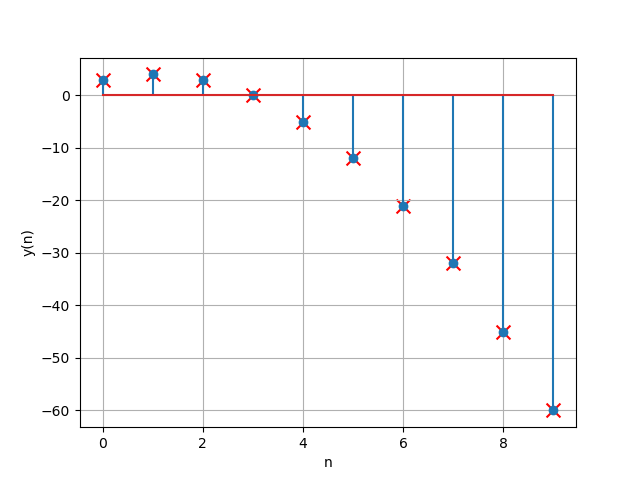
\includegraphics[width=\columnwidth]{figs/main.png}
\caption{\large{stem plot of y(n)}}
\end{figure}
\end{document}
